\documentclass[12pt]{article}
% This file is in the UTF-8 encoding (codepage)
% If you see strange symbols instead of cyrillic letters,
% just switch your editor to UTF-8
% This will not affect the main part of your autoref,
% because the file is inserted as a single separate PDF
% (see below)

\usepackage [utf8]{inputenc}
\usepackage[T2A,T1]{fontenc}

\usepackage[russian]{babel}
\usepackage{amssymb,latexsym,amsmath}
\usepackage{amsfonts}
\pagestyle{plain} \textwidth=185mm \textheight=240mm
\voffset=-17mm \hoffset=-22mm
\renewcommand{\baselinestretch}{1.3}


% Для вставки подписи учёного секретаря
\usepackage{graphics}
\usepackage[dvips]{graphicx}

\begin{document}
\large

\thispagestyle{empty}

% Это не трогаем, пишется всегда
\begin{flushright}
\textit{На правах рукописи}
\end{flushright}

\vspace{25mm}

\begin{center}
\textbf{
	Авдеев Николай Николаевич
}
\end{center}

\vspace{25mm}

\begin{center}
\textbf{\MakeUppercase{
	% Название диссертации :)
	Инвариантные банаховы пределы
}}
\end{center}

\vspace{10mm}

\begin{center}
	1.1.1. Вещественный, комплексный и функциональный анализ
	%1.1.2. Дифференциальные уравнения и математическая физика
\end{center}

\vspace{5mm}

\begin{center}
Автореферат

диссертации на соискание ученой степени кандидата

физико-математических наук
\end{center}

% И с размаху прижимаем вниз!
\vfill

\begin{center}
Москва --- 2025
%Всегда указывается город защиты - Москва
%Независимо от города написания диссертации
\end{center}


\newpage
\thispagestyle{empty}

% Поджимаем междустрочный интервал - а то не влезет!
\renewcommand{\baselinestretch}{1}
% Отключаем абзацные отступы
\setlength{\parindent}{0pt}
% Уменьшем размер шрифта :(
\fontsize{13.4}{15}\selectfont

\begin{center}
	Работа выполнена в
	% Ниже вписываем название университета
	Воронежском государственном университете
\end{center}

\vspace{10mm}



\begin{minipage}[t]{7cm}
	Научный руководитель:
\end{minipage}
%
\begin{minipage}[t]{10cm}

доктор физико-математических наук,

профессор Семенов Евгений Михайлович

\end{minipage}

\vspace{10mm}

Официальные оппоненты:

\hspace{25mm}доктор физико-математических наук,

\hspace{25mm}((TODO)).

\vspace{10mm}

\hspace{25mm}((TODO)) физико-математических наук,

\hspace{25mm}((TODO)).


\bigskip

Ведущая организация - ((TODO))

\vspace{10mm}

TODO: внести реальные дату и время защиты!
\\
Защита состоится 21.12.2025 г. в 15:00 минут
на заседании диссертационного совета
ПДС 0200.005 при Российском университете дружбы народов имени Патриса Лумумбы
(адрес: г. Москва, ул. Орджоникидзе, д. 3).

\vspace{5mm}

С диссертацией можно ознакомиться в
Учебно-научном информационном библиотечном центре
(Научной библиотеке Российского университета дружбы народов)
по адресу: 117198, г. Москва, ул. Миклухо-Маклая, д. 6
и на сайте РУДН в сети <<Интернет>>
(https://www.rudn.ru/science/dissovet).

\vspace{10mm}

Автореферат разослан \_ \_ \_ TODO 2024 г.

\vspace{10mm}


% Прижимаем вниз с размаху!
\vfill

\noindent
\begin{minipage}{0.97\linewidth}
\noindent
Ученый секретарь диссертационного совета
\\
доктор физико-математических наук
\hfill
А. Ю. Савин
\end{minipage}
% Вставляем подпись - и впрямь "посверху"
\nolinebreak
\hspace{-5.8cm}
\begin{minipage}{0.97\linewidth}
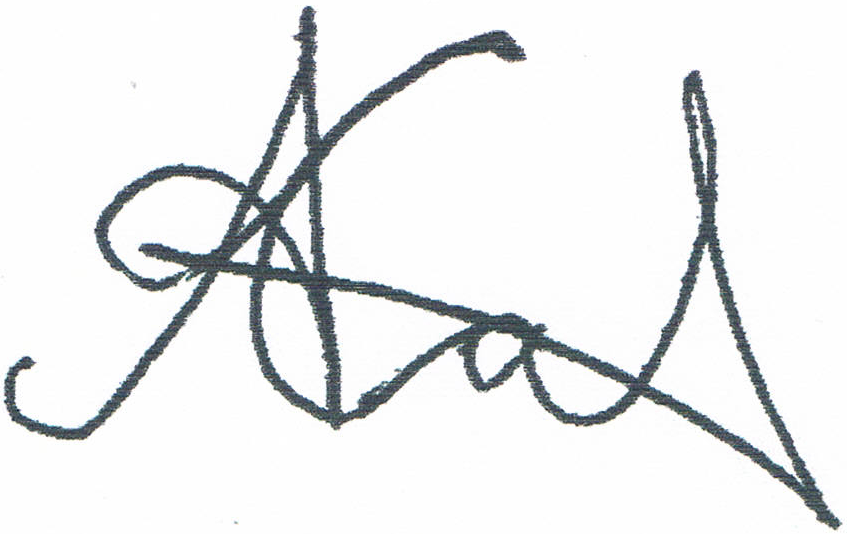
\includegraphics[width=0.10\linewidth]{Savin_signature.png}
\end{minipage}

%...но не совсем вниз...
\vspace{2cm} % по вкусу



\end{document}
